\chapter{Ausblick}\label{ch:ausblick}
Je weiter das Projekt dem Abschluss näher kam desto mehr kristallisierte sich ein Hauptproblem heraus.
Dieses Template ist sehr auf die DATEV Rechnungsschreibung spezialisiert, dass heißt es ist funktionsfähig, aber kann nicht ohne zeitaufwendige Eingriffe in das Template, in die Workflowdefinitionsdateien und die eigentlichen REXX Skripte und Jobs, an eine andere Anwendung angepasst werden.
Zusätzlich ist der durch den momentanen Stand des Templates ermöglichte Bereitstellungsprozess nicht optimal.
Bei der Betrachtung des Falles, wenn zwei Anwender jeweils eine eigene Instanz des gleichen Templates benötigen, muss dieses kopiert werden und neu in z/OSMF aufgenommen werden.
Dies verlangt Wissen über die z/OSMF Oberfläche und den Speicherort des Templates, um es schließlich auch ändern zu können.
Hinzu kommt, dass die Bereitstellung eines IBM Queue Managers nicht im Template enthalten ist.
So müsste dafür ebenfalls ein neuer IBM Queue Manager manuell angelegt werden.
Eine Herangehensweise an dieses Problem wird im Folgenden beschrieben.
Diese ist als Ausblick zu verstehen, die Umsetzung ist kein Bestandteil dieser Arbeit.

Angenommen das Template beinhaltet die Provisionierung eines IBM Queue Managers.
So könnte jeder Mitarbeitern seine eigene Instanz des Templates besitzen und beispielsweise für eigene Tests nutzen.
Da die Application Id einer CICS-Instanz eindeutig sein muss, müsste dennoch jeder Mitarbeiter ein eigenes Template dahingehend anpassen, dass dies gewehrleistet ist.
Eine Möglichkeit wäre eine Definition eines Pools mit verfügbaren Application Ids und dann mittels eines Programmes eine ungenutzte zu bestimmen.
Dieses Programm kann dann in das Template mittels eines Steps aufgenommen werden.
Das würde das Problem mit der eindeutigen Application Id lösen.
Jedoch müsste immer noch für jede kleine Änderung an der Konfiguration des Templates ein neues erzeugt werden.
Hier schafft z/OSPT Abhilfe.
Damit kann, wie in Absatz \ref{sssec:zospt} beschrieben, mit Hilfe einer Konfigurationsdatei das Template von außerhalb gesteuert werden.
Dadurch fällt das Kopieren des Template für den Mitarbeiter weg, dieser muss mittels des Kommandozeileninterfaces ein Image bauen und daraus einen Container erzeugen.
Das Kommandozeileninterface hat einen weiteren Vorteil.
Mit Hilfe von diesem können diese Arbeitsschritte in eine Jenkins-Ablauf aufgenommen werden.
Somit läuft der Prozess automatisiert ab und nähert sich modernen Entwicklungsabläufen an.

Die Arbeitsweise und der Bereitstellungsprozess für die Laufzeitumgebung, die der DATEV Rechnungsschreibungs-Ablauf benötigt, ist dadurch vereinfacht und es werden weniger Absprachen benötigt.
Allerdings ist das Template weit von einer Nutzung außerhalb der DATEV Rechnungsschreibung entfernt.
Während der Realisierung dieser Arbeit wurde klar, dass anwendungsspezifische Templates nicht optimal sind und nicht den vollständigen Funktionsumfang von `IBM Cloud Provisioning and Management for z/OS` ausreizen.
So ist zu empfehlen, dass für jedes Subsystem, also CICS, Db2 und IBM MQ, ein eigenständiges Template zu realisieren ist.
Für die Realisierung davon müssten die Template dynamischer implementiert sein.
Um dies zu verdeutlichen wird als Beispiel die Provisionierung von IBM MQ Queues herangezogen.
Momentan werden die Prozesse und die Trigger Queues sehr statisch angelegt.
Das heißt, dass sowohl Namen als auch die damit verknüpften Queueparameter fest hinterlegt sind.
Um nur ein Beispiel zu nennen.
Dies müsste dahingehend angepasst werden, dass alle Parameter in einer Konfigurationsdatei angeben werden können.
Es ist auch in Betracht zu ziehen, ob für den User nur bestimmte vorgefertigte Profile, wie \glqq klein\grqq, \glqq mittel\grqq{} und \glqq groß\grqq, auswählbar sind.
Dies müsste alles in dem Template implementiert werden.
Hierfür ist noch viel Zeitaufwand von Seiten der Administration einzuplanen.

Angenommen es existieren jeweils ein CICS, ein Db2 und ein IBM MQ Template und diese sind so realisiert, dass sie firmenweit eingesetzt werden können.
Dann ist der nächste Schritt, die Aufnahme in den \glqq DATEV Marktplatz\grqq, möglich.
Der \glqq DATEV Marktplatz\grqq{} ist eine Weboberfläche mit der sich Entwicklerteams ihre benötigte PaaS-Umgebung konfigurieren können.
Heute stehen ihnen dort Dienste wie MongoDB, PostgreSQL, Kafka und viele weitere zur Verfügung.
In weiter Zukunft könnten hier auch Dienste wie CICS, Db2 und IBM MQ zur Auswahl stehen.
Im Hintergrund würden diese über Templates und Images Instanzen bereitstellen.
Um dies zu verwirklichen könnte die von z/OSMF zur Verfügung gestellte REST-API verwendet werden.
Diese ermöglicht den Zugriff auf fast alle z/OSMF Funktionalitäten mittels Requests.
Für die \glqq Tenant\grqq{} Zuweisung zu einem Template existiert noch kein Request.
Daran ist zu erkennen, dass von Seiten von z/OSMF beziehungsweise von IBM ebenfalls noch Verbesserungsmöglichkeiten bestehen.

Diese technische Umsetzung ermöglicht in Zukunft den in Diagramm \ref{fig:proneu} dargestellten Bereitstellungsprozess.
Es ist zu erkennen, dass Verantwortung von den Administratorenteams an die Entwicklerteams übertragen wird.
Dadurch wird Kommunikationsaufwand eingespart und einem Entwickler steht binnen weniger Minuten eine funktionsfähige Laufzeitumgebung für seine legacy z/OS Anwendung zur Verfügung.
Bei Problemen oder Beratungswunsch unterstützen die Administratorenteams weiterhin.

\begin{figure}[ht!]
\centering
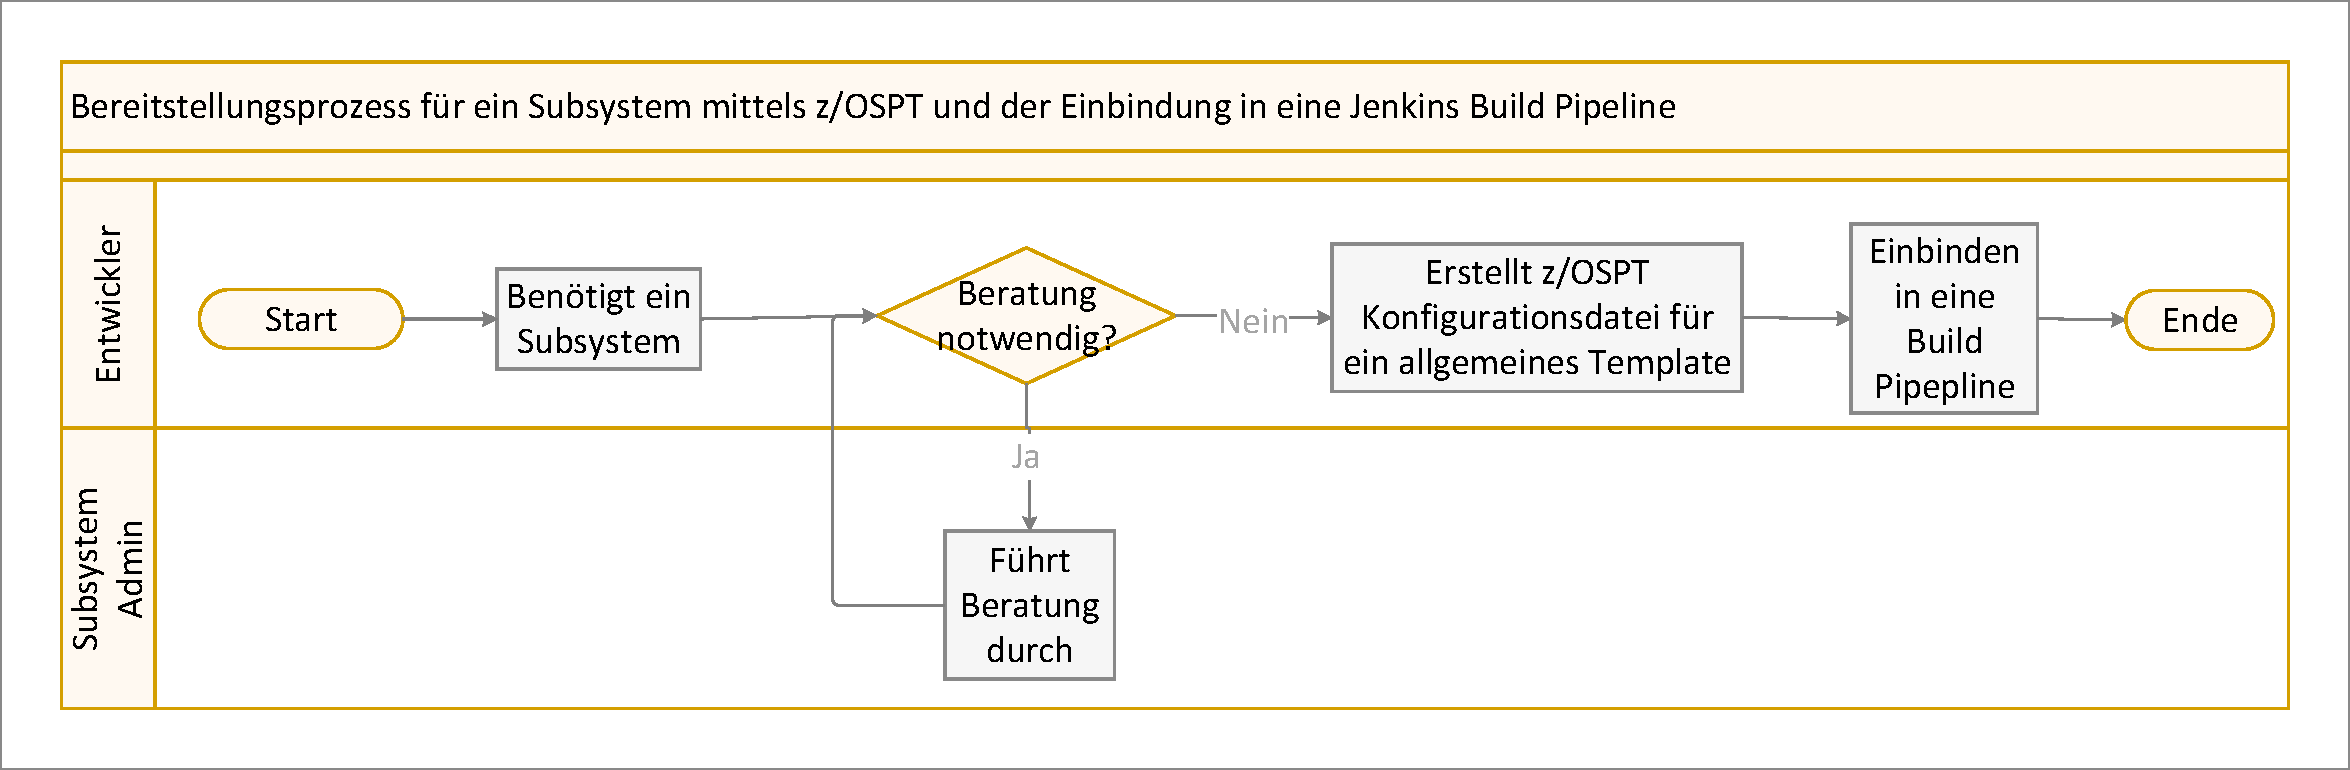
\includegraphics[width=\paperwidth,angle=90]{figures/swimlaneNeuerProzess.pdf}
\caption{Bereistellungsprozess eines Subsystems mittels einer z/OSPT Konfigurationsdatei}
\label{fig:proneu}
\end{figure}


